\documentclass[a4paper,12pt]{article}

\usepackage{geometry}
\geometry{top=15mm}
\geometry{bottom=30mm}
\geometry{left=10mm}
\geometry{right=20mm}
\linespread{1}
\setlength{\parindent}{12pt}
\setlength{\parskip}{8pt}

\usepackage{titleps}

\newpagestyle{main}
{
  \setheadrule{0.4pt}
  \sethead{}{}{}
  \setfootrule{0,4pt}
  \setfoot{}{\thepage}{}
}
\usepackage{color}
\usepackage[english,russian]{babel}
\usepackage[T2A]{fontenc}
\usepackage[utf8]{inputenc}
\usepackage{amsthm,amsmath,amsfonts,amssymb,mathtools}
\usepackage{indentfirst}
\usepackage{lipsum}
\usepackage{graphicx}
\usepackage{float}
\usepackage{wrapfig}

\newcommand{\partdef}[2]{\frac{\partial \mathnormal{#1}}{\partial \mathnormal{#2}}}






\newcommand{\Arctan}[1]{ \mathcal{Arctan(}\mathnormal{#1}\mathca{)} }


\begin{document}

\section{Аналитическое решение задачи.}

Отыскание общего решения данной системы является достаточно тяжелой задачей, поэтому наша цель будет найти такие решения, которые удовлетворяютя данной системе. Итак, имеем следующую систему уравнеий:

\begin{align*}
    &\left\{
        \begin{array}{l}
            \dot x =y,\\
            \dot y= u,\\
            \dot p_x= 0\\
            \dot p_y= -p_x -\frac{2\cdot t^r \cdot y}{{(1+y^2)}^2}\\
            u=\left\{
            \begin{array}{l}
                16 \text{ ,если } p_y>0 \\
                0 \text{ ,если } p_y<0
            \end{array}
            \right.
        \end{array}
    \right.
    \\
    &\begin{array}{l}
        x(0)=0, \: x(2)=1,\\
        p_y(0)=0, \: p_y(2)=0,\\
        r \in \{1, 2\}.
    \end{array}
\end{align*}

Задаем начальные условия:
\begin{align}
    x(0)=0\:\:,\:\:y(0)=y_0\:\:,\:\:p_y(0)=0\:\:,\:\:p_x(0)=p_x^0.
\end{align}

Решим для начала задачу с параметром $r=1.$

\textbf{Будем считать, что $p_x^0 > 0.$} Тогда имеем $\dot p_y(0)<0$, что означает, что необходимо выставить параметр $u=0.$. Решая эту систему уравнеий получаем следующие решения:

\begin{align*}
    \left\{
        \begin{array}{l}
            x(t)\;=\; y_0\cdot t\\
            y(t)\; \equiv \; y_0\\
            p_x(t)\;\equiv \; p_x^0\\
            p_y(t)\; =\; -p_x^0\cdot t\;-\;\frac{y_0}{(1+y_0^2)^2\cdot t^2}
        \end{array}
    \right.
\end{align*}

Пусть $t^*$ - момент, когда $p_x(t^*)\;=\;0\;.$ Заметим лишь, что если $y_0\;=\; 0$ , то имеем противоречие  с $p_y(2)=0$.
Тогда для этого момента времени справедливо:

\begin{align*}
    \left\{
        \begin{array}{l}
            x(t^*)\;=\;   y_0\cdot t^*\\
            y(t^*)\;=\;   y_0\\
            p_x(t^*)\;=\; p_x^0\\
            p_y(t^*)\;=\; 0
        \end{array}
    \right.
    \;\;\; \text{,где  } t^* \;=\; \frac{p_x^0 \cdot (1+y_0^2)^2}{- y_0 } . 
\end{align*}

\begin{align*}
&t^* \;>\; 0 \Rightarrow y_0\;<\;0\;\\
&t^* \in \left(0\:,\:2\rigth] \text{ , причем если } t^* \;=\; 2 \text{ , то имеем противоречие с } x(2)=1; \;\Rightarrow\; \\
& \;\Rightarrow\; t^* \in \left(0\:,\:2\right) \Leftrightarrow  \;0\;<\; p_x^0\; < \; \frac{-2 \cdot y_0}{(1+y_0^2)^2}
\end{align*}

Заметим, что $\dot p_y(t^*)=p_x^0 \;>\;0 $ , что означает, что решение переходит в верхнюю полуплоскость трансверсально, поэтому после точки $t^*$ считаем $u=16$ . Для удобства совершим сдвиг по оси времени $t\;=\;\tau + t^*$, и тогда  новая систеа примет следующий вид:

\begin{align*}
    \left\{
        \begin{array}{l}
            \dot x\;=\; y,\\
            \dot y\;=\; u,\\
            \dot p_x\;=\; 0\\
            \dot p_y\;=\; -p_x -\frac{2\cdot (\tau + t^*) \cdot y}{{(1+y^2)}^2}\\
        \end{array}
    \right.
\;\;\; \text{, с начальными условиями }
    \left\{
        \begin{array}{l}
            x(0)\;=\;   y_0\cdot t^*\\
            y(0)\;=\;   y_0\\
            p_x(0)\;=\; p_x^0\\
            p_y(0)\;=\; 0
        \end{array}
    \right.
\end{align*}

Решаем эту систему уравнений и получаем следующее решение:
\begin{align*}
    \left\{
        \begin{array}{l}
            x(\tau)\;=\; 8 {\tau}^{2}+\tau \cdot y_0 + y_0 \cdot t^*\\
            y(\tau)\;=\; 16 \tau + y_0\\
            p_x(\tau)\;=\; p_x^0\\
            p_y(\tau)\;=\; \frac{1}{256}\left(
                16 \left(
                    -16\cdot p_x^0 \cdot \tau - \frac{t^*}{1+y_0^2} + \frac{\tau + t^*}{1+(16 \cdot \tau + y_0)^2}
                \right)+
                \mathbf{Arctan}(y_0)-
                \mathbf{Arctan}(16 \tau + y_0)
            \right)
        \end{array}
    \right.
\end{align*}

Попытаемся найти такие начальные значения, что будут выполнены краевые условия, то есть:

\begin{align*}
    \left\{
        \begin{array}{l}
            x(2-t^*)\;=\;1 \\
            p_y(2-t^*)\;=\;0
        \end{array}
    \right.
    \;\;\;\text{ , причем } p_x^0 \;=\; -\frac{t^* \cdot y_0}{(1+y_0^2)^2}
    \\
    x(2-t^*)\;=\;1\; \Rightarrow \; t^*\;=\;2\;\pm \frac{\sqrt{2}}{4}\sqrt{1-2\cdot y_0}\text{ , }
    \\
    \text{ также необходимо вспомнить об ограничении }t^*\in\left(0,2\right)\text{ ,}
    \\
    \left[
    \begin{array}{l}
        t^*\;=\;2\;+ \frac{\sqrt{2}}{4}\sqrt{1-2\cdot y_0}\;>2\;\text{ для }\forall y_0\;<\;0\text{ -противоречие.}
        \\
        t^*\;=\;2\;- \frac{\sqrt{2}}{4}\sqrt{1-2\cdot y_0}\;\Rightarrow\; -\frac{31}{2}\;<\;y_0\;<\;0
    \end{array}
    \right.
    \\
    \text{подставляя соответствующие функции в последнее уравннение системы }\Rightarrow 
\end{align*}

\begin{multline*}
    \frac{4(-8+\sqrt{2-4\cdot y_0})}{1+y_0^2}+{}\\
    {}+32 \cdot \frac{\sqrt{2-4\cdot y_0}(132\cdot y_0-264\cdot y_0^2+20\cdot y_0^3)+(1-33\cdot y_0+196\cdot y_0^2-257\cdot y_0^3+3\cdot y_0^4)}{(1+y_0^2)^2\cdot (33+8(-8+\sqrt{2-4 \cdot y_0})\cdot y_0 +y_0^2)}+{}\\
    {}+\mathbf{Arctan}(y_0)-
    \mathbf{Arctan}(4\sqrt{2-4\cdot y_0}+ y_0)\;=\; 0
\end{multline*}

\begin{wrapfigure}{r}{0.4\textwidth}
    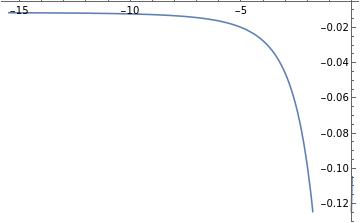
\includegraphics[width=0.4\textwidth]{img1.png}
\end{wrapfigure}

Из рисунка видно, что последнее уравнение не разрешимо на промежутке $-\frac{31}{2}\;<\;y_0\;<\;0$ .
Причем из рисунка также видно, что $p_y(2-t^*)$ в зависимости от $y_0$ может принимать как положительные, так и отрицатеьные значения, поэтому опять найдется точка переключения со своими ограничениями. После точки переключения управление $u\;=\;0$ .

Это породит новую систему уравнений со своими начальными условиями, с учетом сдвигом по времени эту систему можно записать так:

Для удобства введем обозначения $t_1\:=\: t^*$ , $t_2$ -момент времени, когда посленяя функция $p_y(t2)\;=\;0$ . 

\begin{align*}
    \left\{
        \begin{array}{l}
            \dot x\;=\; y \\
            \dot y \;=\;0 \\
            \dot p_x \;=\;0\\
            \dot p_y \;=\; -p_x - \frac{2\cdot (t+t_1+t_2)\cdot y}{(1+y^2)^2}
        \end{array}
    \right.
    \text{  ,}
\end{align*}
с начальными условиями 
\begin{align*}
    \left\{
        \begin{array}{l}
            x(0)\;=\; x_2 \\
            y(0) \;=\; y_2 \\
            p_x(0) \;=\; p_x^0\\
            p_y(0) \;=\; 0
        \end{array}
    \right.
    \;\;\; \text{ , где }
    \left\{
        \begin{array}{l}
            x_2\;=\; 8 t_2^2 + t_2\cdot y_0 + y_0 \cdot t_1 \\
            y_2 \;=\; 16 t_2 + y_0 \\
            t_1 \;=\; \frac{p_x^0 \cdot (1+y_0^2)^2}{- y_0 }
        \end{array}
    \right.
\end{align*}
Далее хотим разрешить краевую задачу.  Решение системы уравнений примет вид:
\begin{align*}
    \left\{
        \begin{array}{l}
            x(t)\;=\; x_2\cdot t +x_2 \\
            y(t) \;=\; y_2 \\
            p_x(t) \;=\; p_x^0\\
            p_y(t) \;=\; t\left( -p_x^0 - \frac{2\cdot (t_1 + t_2)\cdot y_2}{(1+y_2^2)^2}-\frac{t^\cdot y_2}{(1+y_2^2)^2} \right)=t\cdot \psi(t,t_2,t_1,y_2,p_x^0)
        \end{array}
    \right.
\end{align*}

Опишем идею построения уравнений :

\begin{align*}
\left.
\begin{array}{l}
    \left.
    \begin{array}{l}
        t_1\:=\:t_1(y_0,p_x^0) \Rightarrow p_x^0\:=\:p_x^0(y_0,t_1)
        \\
        \left.
        \begin{array}{l}
                y_2 \:=\: y_2(y_0,t_2)\\
                x_2 \:=\: x_2(t_2,t_1,y_0)\\
                x(2-t_1-t_2)\:=\: \phi(y_2,x_2,t_1,t_2) \:=\:1
        \end{array}
        \right\} \Rightarrow t_1 \:=\: t_1(t_2,y_0)
    \end{array}
    \right\} \Rightarrow p_x^0\:=\:p_x^0(y_0,t_2)
    \\
    \psi(2-t_1-t_2,t_2,t_1,y_2,p_x^0)\:=\:0
\end{array}
\right\} \Rightarrow f(t_2,y_0)\:=\:0 .
\end{align*}

\begin{wrapfigure}[10]{l}[26pt]{0.4\textwidth}
    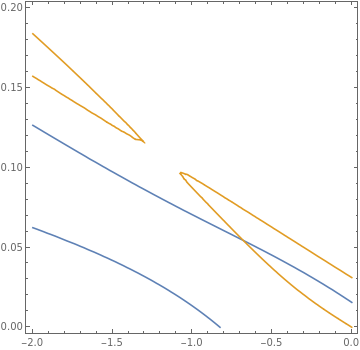
\includegraphics[width=0.4\textwidth]{img2.png}
    \caption{
        \begin{array}{r}
            y_0=-0.681078049\\
            t_2=0.054491750283
        \end{array}
        }
\end{wrapfigure}


А также вспоминая предшествующее уравнение $p_y(t_2)=0 \Leftrightarrow G(t_2,t_1,y_0,p_x^0)\:=\:0$ и совершая аналогичный ряд действия, имеем:

\begin{align*}
    \begin{array}{l}
            f(t_2,y_0)\:=\:0
            \\
            g(t_2,y_0)\:=\:0
    \end{array}
\end{align*}

Было найда пара точек (рис.1 и рис.2), которые могут претедовать на решение, но не одна из точек не подхоит, так как вычесленное по ним время $t_1 \:<\:0$ .

\newpage


\begin{wrapfigure}[15]{l}[26pt]{0.4\textwidth}
        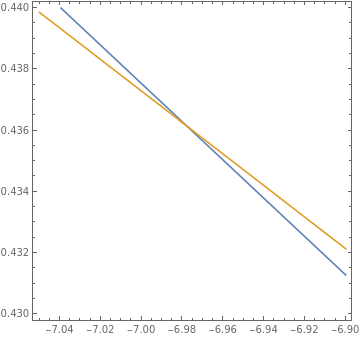
\includegraphics[width=0.4\textwidth]{img3.png}
        \caption{
            \begin{array}{r}
                y_0=-6.977892188\\
                t_2=0.43614901116
            \end{array}
            }
\end{wrapfigure}
Таким образом мы можем далее искать точку переключения и продолжать решение, но это уже сложная задача, поэтому будем пытаться найти решение среди других начальных параметров.

\textbf{Далее будем считать, что $p_x^0=0$ .} 
Заметим, что $y(0)=y_0 \neq 0$, так как решения, тождественно равные 0 нас не интересуют. Таким образом задача распадается на два случая:

Пусть $y_0 > 0$ . Тогда для достаточно маленьково $\delta$ верным будет утверждение, что $\dot p_y(\tau) < 0$ на всем промежутке $\left(0,\delta \right)$. Так как $p_y(0)=0$ , то необходимо брать $u=0$. Это приведет к тому, что:
\begin{align*}
    p_y(t)=&\frac{- t^2\cdot y_0}{(1+y_0^2)^2} \Rightarrow \\ & \nexists \text t_1\text{ , что }p_y(t_1)=0\text{ , что приводит к противоречию.}
\end{align*}
Пусть $y_0 < 0$ . Тогда для достаточно маленьково $\delta$ верным будет утверждение, что $\dot p_y(\tau) > 0$ на всем промежутке $\left(0,\delta \right)$. Так как $p_y(0)=0$ , то необходимо брать $u=16$. Это приведет к тому, что:

\begin{align*}
    p_y(t)=\frac{\mathbf{Arctan}(y_0)-\mathbf{Arctan}(16\cdot t+y_0)}{256}+\frac{t}{16(1+(16\cdot t+y_0)^2)}
    \\
    \begin{array}{c}
        x(t)=8 t^2+t\cdot y_0 \text{ , требуем, чтобы }p_y(2)=0 \text{ и }x(2)=1 .
        \\
        x(2)=1 \; \Rightarrow \; y_0=-\frac{31}{2} \; \Rightarrow \; p_y(2) \neq 0.
    \end{array}
\end{align*}

Это означает, что следует искать точку переключения $t_1$ , затем строить новую систему уравнений и ее решать, в ходе чего будет получено:
Для удобства считаем, что произошел сдвиг по времени.
\begin{align*}
    p_y(t)=\frac{- t^2\cdot y_1}{(1+y_1^2)^2}\text{ , где }y_1=16*t_1+y_0.
\end{align*}
Таким образом имеем, что необходимо выполение $y_1=0$ , иначе невозможно выполнение краевых условие. Тогда имеем уравнение $t_1=t_1(y_0)$ , подстановка которого в $p_y(t_1)=0$ ,полученного на первом шаге дает противоречие, значит решение вообще невозможно при $p_x^0=0$.

\textbf{ Тогда разберемся с последним случаем $p_x^0<0$ .}

\begin{wrapfigure}[11]{r}[26pt]{0.4\textwidth}
    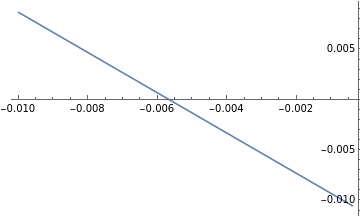
\includegraphics[width=0.4\textwidth]{img4.png}
    \caption{$p_x^0=-0.00566313$}
\end{wrapfigure}

Тогда $\dot p_y(0)>0$ , и в качестве параметра необходимо взять $u=16$ . Тогда получим систему, решением которого имеет вид:

\begin{align*}
    \left\{
        \begin{array}{l}
            x(t)=8 t^2\cdot y_0\\
            y(t)=16 t+y_0\\
            p_x(t) \equiv p_x^0\\
            p_y(t)=-p_x^0\cdot t+\frac{\mathbf{Arctan}(y_0)-\mathbf{Arctan}(16\cdot t+y_0)}{256}+\frac{t}{16(1+(16\cdot t+y_0)^2)}
        \end{array}
    \right.
\end{align*}
Тогда попытаемся решыть такую систему:
\begin{align*}
    \begin{array}{l}
        x(2)=1\;\Rightarrow \; y_0=-\frac{31}{2}\\
        p_y(2)=0\text{ , при} y_0=-\frac{31}{2} \; \Rightarrow \; p_x^0=-0.00566313
    \end{array}
\end{align*}
Таким образом мы нашли решение, не имеющее точки переключения с начальными параметрами $(p_x^0,y_0)=(-0.00566313,-\frac{31}{2})$.
\newline
\begin{wrapfigure}[15]{l}[26pt]{0.4\textwidth}
    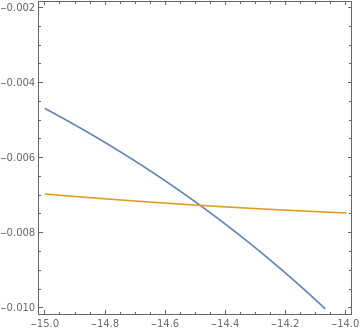
\includegraphics[width=0.4\textwidth]{img5.png}
    \caption{
        \begin{array}{l}
            $p_x^0=-0.00725785633$\\
            $y_0=-14.4849204322$
        \end{array}
        }
\end{wrapfigure}

Попытаемся теперь построить решение, проходящее через одну точку переключения.
Тогда получим новую систему уравнений(с учетом сдвига по времени и сменой значения параметра на 0):


\begin{align*}
    \left\{
        \begin{array}{l}
            \dot x \equiv y_1\\
            \dot y \equiv 0\\
            p_x(t) \equiv p_x^0\\
            \dot p_y=-p_x^0-\frac{2(t+t_1)\cdot y_1}{(1+y_1^2)^2}
        \end{array}
    \right.
    \text{ , где }
    \left\{
        \begin{array}{l}
            x(0) \;=\; x_1 \;=\; 8t_1^2+t_1\cdot y_0\\
            y(0) \;=\; y_1 \;=\; 16t_1+y_0\\
            p_y(0)=0
        \end{array}
    \right.
    \;\;\Rightarrow
    \\
    \\
    \left\{
        \begin{array}{l}
            x(t) \;=\; y_1\cdot t+ x_1\\
            y(t) \;=\; y_1 \\
            p_y(t)=- p_x^0\cdot t-\frac{t^2\cdot y_1}{(1+y_1^2)^2}-\frac{2t\cdot t_1\cdot y_1}{(1+y_1^2)^2}
        \end{array}
    \right.
    \text{ , где }
\end{align*}
\newline
\begin{align*}
    0=-p_x^0\cdot t_1&+\frac{\mathbf{Arctan}(y_0)-\mathbf{Arctan}(16\cdot t_1+y_0)}{256}
    \\
    +&\frac{t_1}{16(1+(16\cdot t_1+y_0)^2)} \Leftrightarrow f_2(y_0,t_1,p_x^0)=0
\end{align*}
\begin{aling*}
    \\
    x(2-t1) \;=\; y_1\cdot (2-t1)+ x_1 \;=\;1 \Rightarrow t_1=\frac{1}{2}(4-\sqrt{16+y_0})
    \\
    \\
    \begin{array}{l}
        \left\{
            \begin{array}{l}
                p_y(2-t_1)=0\\
                t_1=t_1(y_0)\\
                y_1=y_1(y_0,t_1)
            \end{array}
        \right.
        \;\Rightarrow\; F_1(p_x^0,y_0)=0
        \\
        \\
        \left\{
            \begin{array}{l}
                f_2(y_0,t_1,p_x^0)=0\\
                t_1=t_1(y_0)
            \end{array}
        \right.
        \;\Rightarrow\; F_2(p_x^0,y_0)=0
    \end{array}
    \;\Rightarrow\; 
    \left\{
        \begin{array}{l}
            F_2(p_x^0,y_0)=0\\
            F_1(p_x^0,y_0)=0
        \end{array}
    \right.
\end{align*}

Решая эту систему, находим точку $(p_x^0,y_0)=(-0.00725785633,-14.4849204322)$ осталось проверить, что эта точка определяет допустимое $t_1$ .

\begin{align*}
    t_1=\frac{1}{2}(4-\sqrt{16+y_0}) \;\Rightarrow\; t_1=1.384553 \in \left(0,2\right) \;\Rightarrow\;\text{удовлетворяет ограничениям на время.}
\end{align*}

Таким образом мы нашли два решения:

\begin{array}{l}
    $(p_x^0,y_0)=(-0.00566313,-\frac{31}{2})$\text{ - без точек переключения .}
    \\
    $(p_x^0,y_0)=(-0.00725785633,-14.4849204322)$\text{ - с одной точкой переключения.}
\end{array}


\end{document}